\documentclass{article}
\usepackage[left=0.5in,top=0.5in,right=0.5in,bottom=0.5in]{geometry}
\usepackage[english]{babel}
\usepackage[utf8]{inputenc}
\usepackage[table]{xcolor}
\usepackage{amssymb,amsmath,amsthm}
\usepackage{changepage,threeparttable}
\usepackage{booktabs,multirow}
\usepackage{graphicx}
\usepackage{soul}
\graphicspath{{./images/}}
\def\R#1{\(R_{\text{\tiny#1}}\)}
\def\V#1{\(V_{\text{\tiny#1}}\)}
\def\I#1{\(I_{\text{\tiny#1}}\)}
\def\Rr#1{R_{\text{\tiny#1}}}
\def\Vv#1{V_{\text{\tiny#1}}}
\def\RDIV{\(\frac{R_{\text{1}}}{R_{\text{1}}+R_{\text{2}}}\)}
\def\VDIV{\(\frac{V_{\text{1}}}{V_{\text{12}}}\)}
\title{Lab 5: Voltage Divider}
\author{Philip Kim}
\date{\today}
\begin{document}
\maketitle
\vspace*{-1cm}
\begin{table}[!htp]\centering
  \subsection*{Part 1}
  \begin{tabular}{|c|c|c|c|c|c|c|c|}\hline
  \multicolumn{7}{|c|}{\textbf{Table 1: Series Resistors}} \\\hline
  \R{1} & \R{2} & \V{1} & V/DIV for \V{1} & \V{12} & \RDIV\ & \VDIV\ \\\hline
  1k & 2k & 0.68V & 1V & 2.02V & 0.33k & 0.34V \\\hline
  1k & 100 & 1.82V & 1V & 1.98V & 0.91k & 0.92V \\\hline
  1k & 4.7k & 0.40V & 1V & 2.02V & 0.18k & 0.2V \\\hline
  1k & 10k & 0.28V & 1V & 2.02V & 0.09k & 0.14V \\\hline
  1k & 100k & 0V & 0V & 0V & 0.01k & 0 \\\hline
  \end{tabular}
  \begin{center}
    \subsection*{Picture 1: }
    % 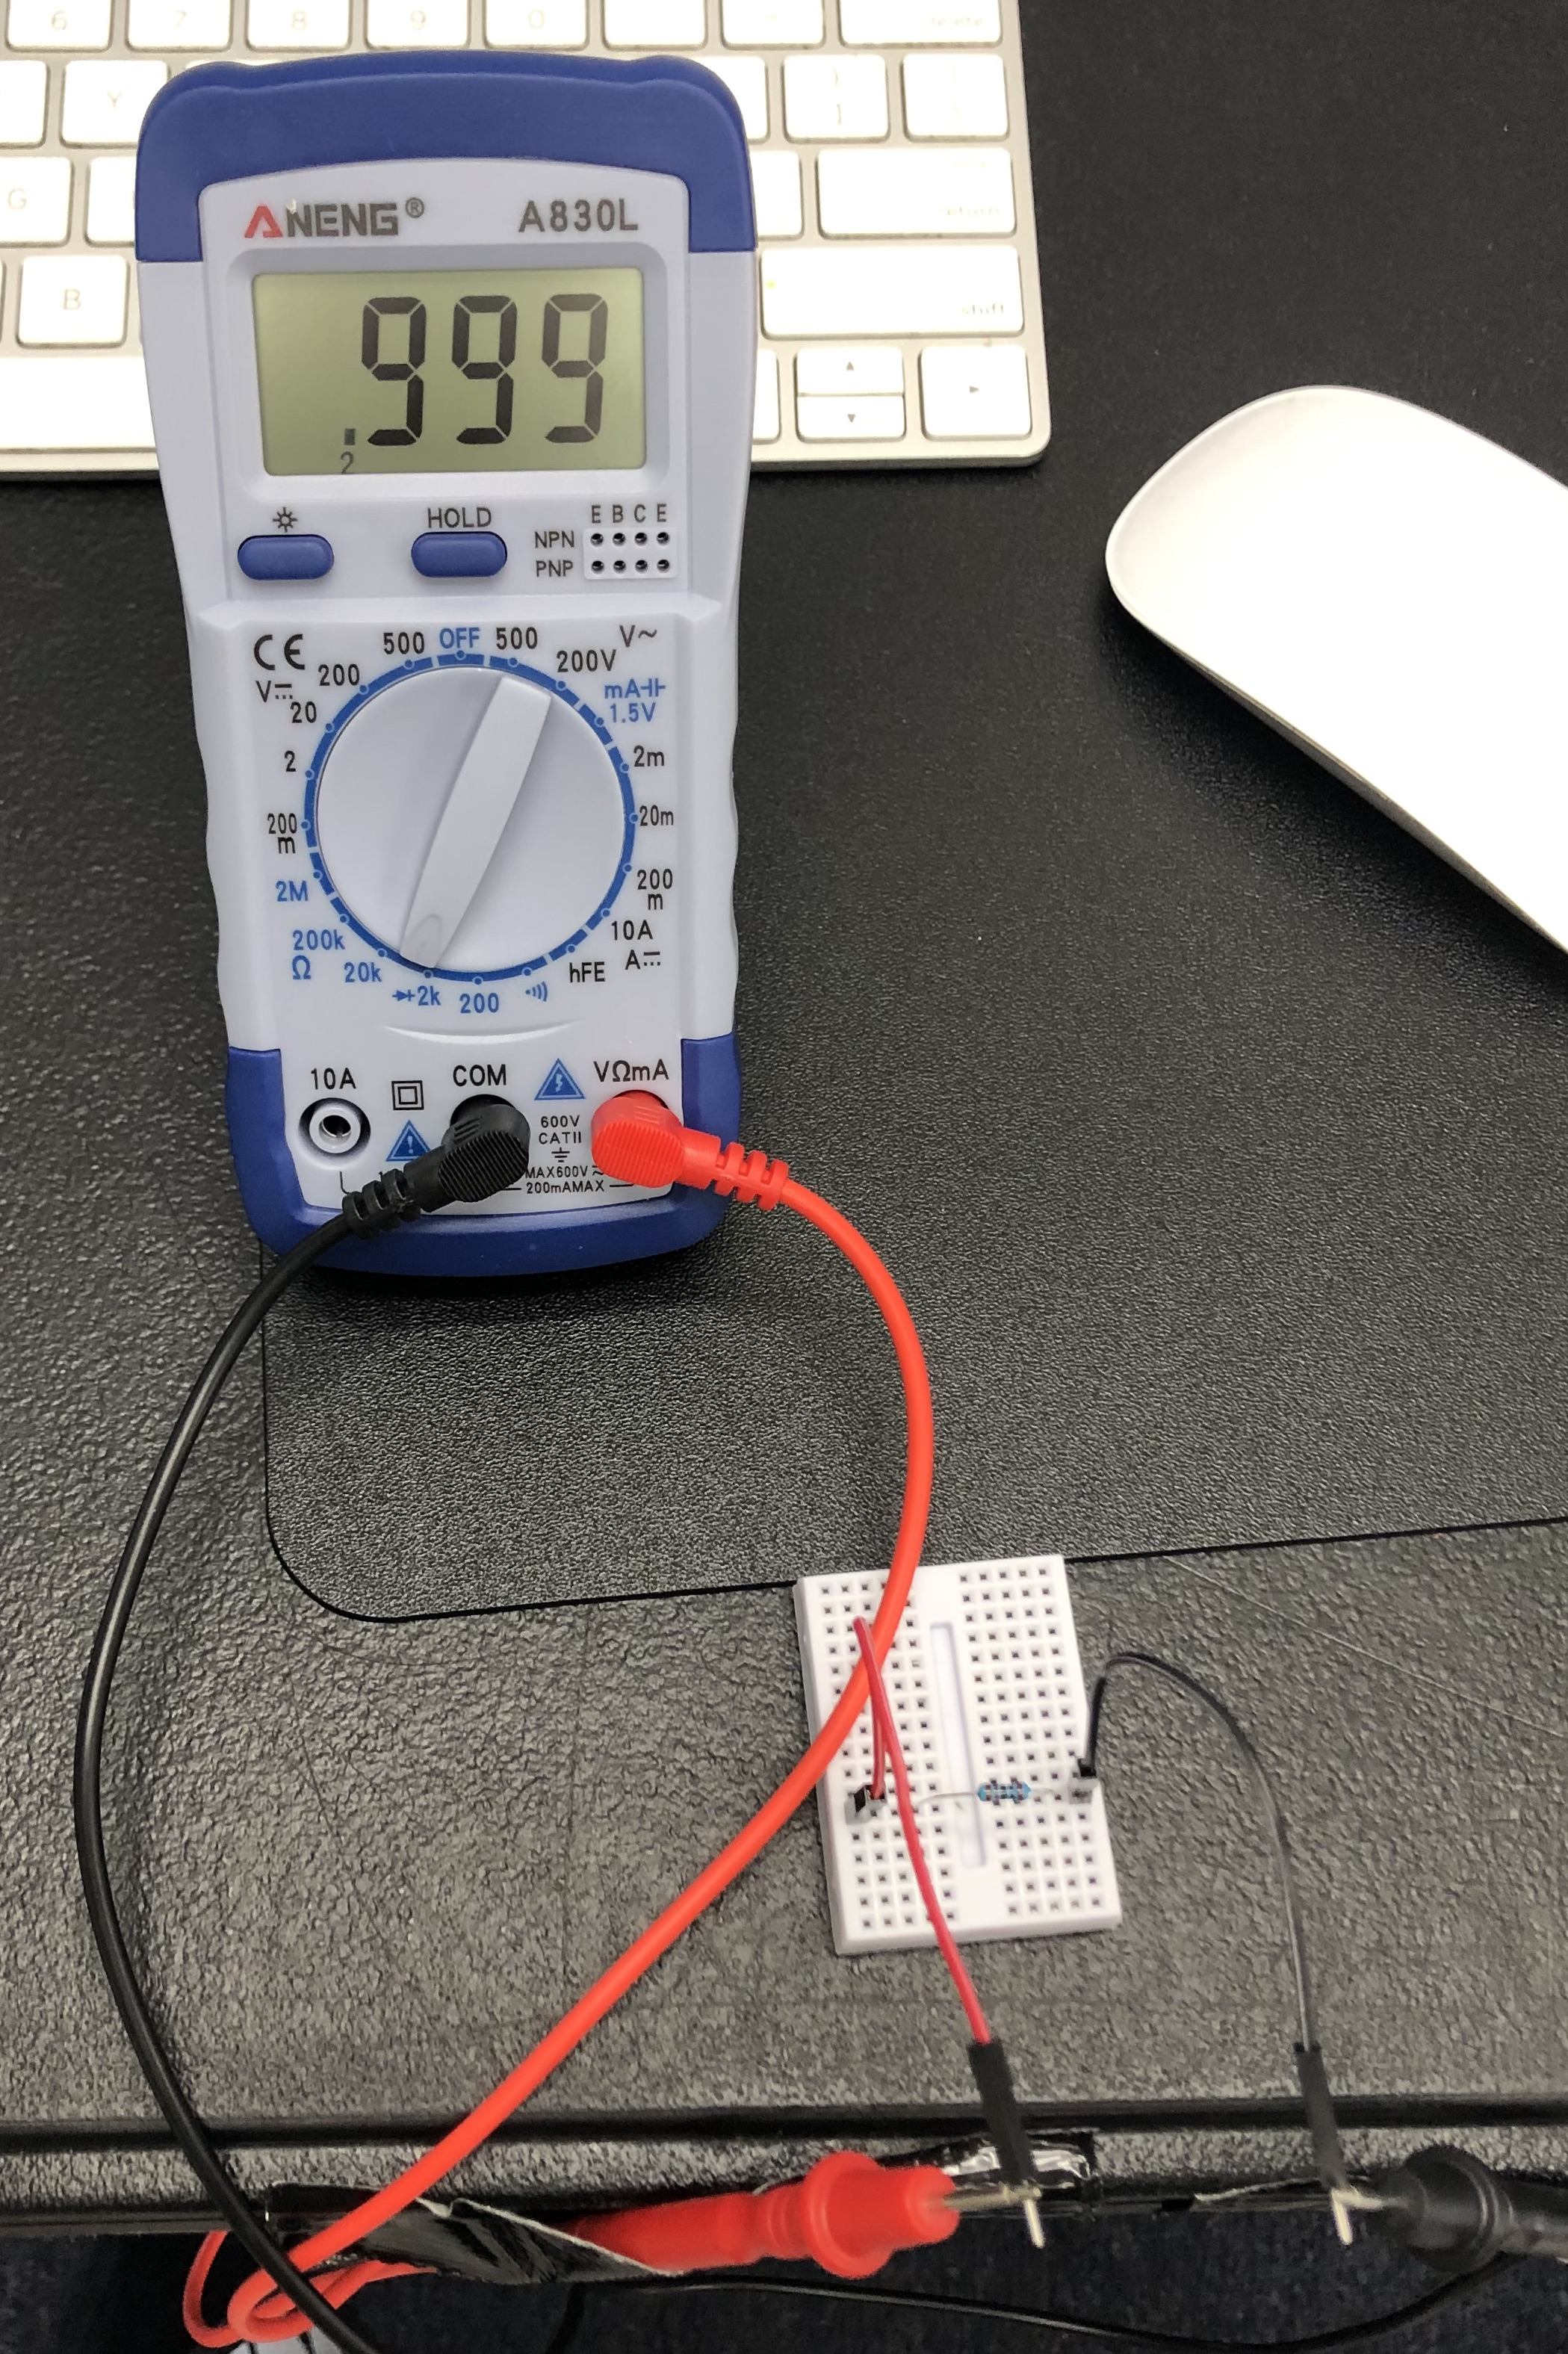
\includegraphics[scale=0.079,height=4.5cm]{R1.jpeg}
    % 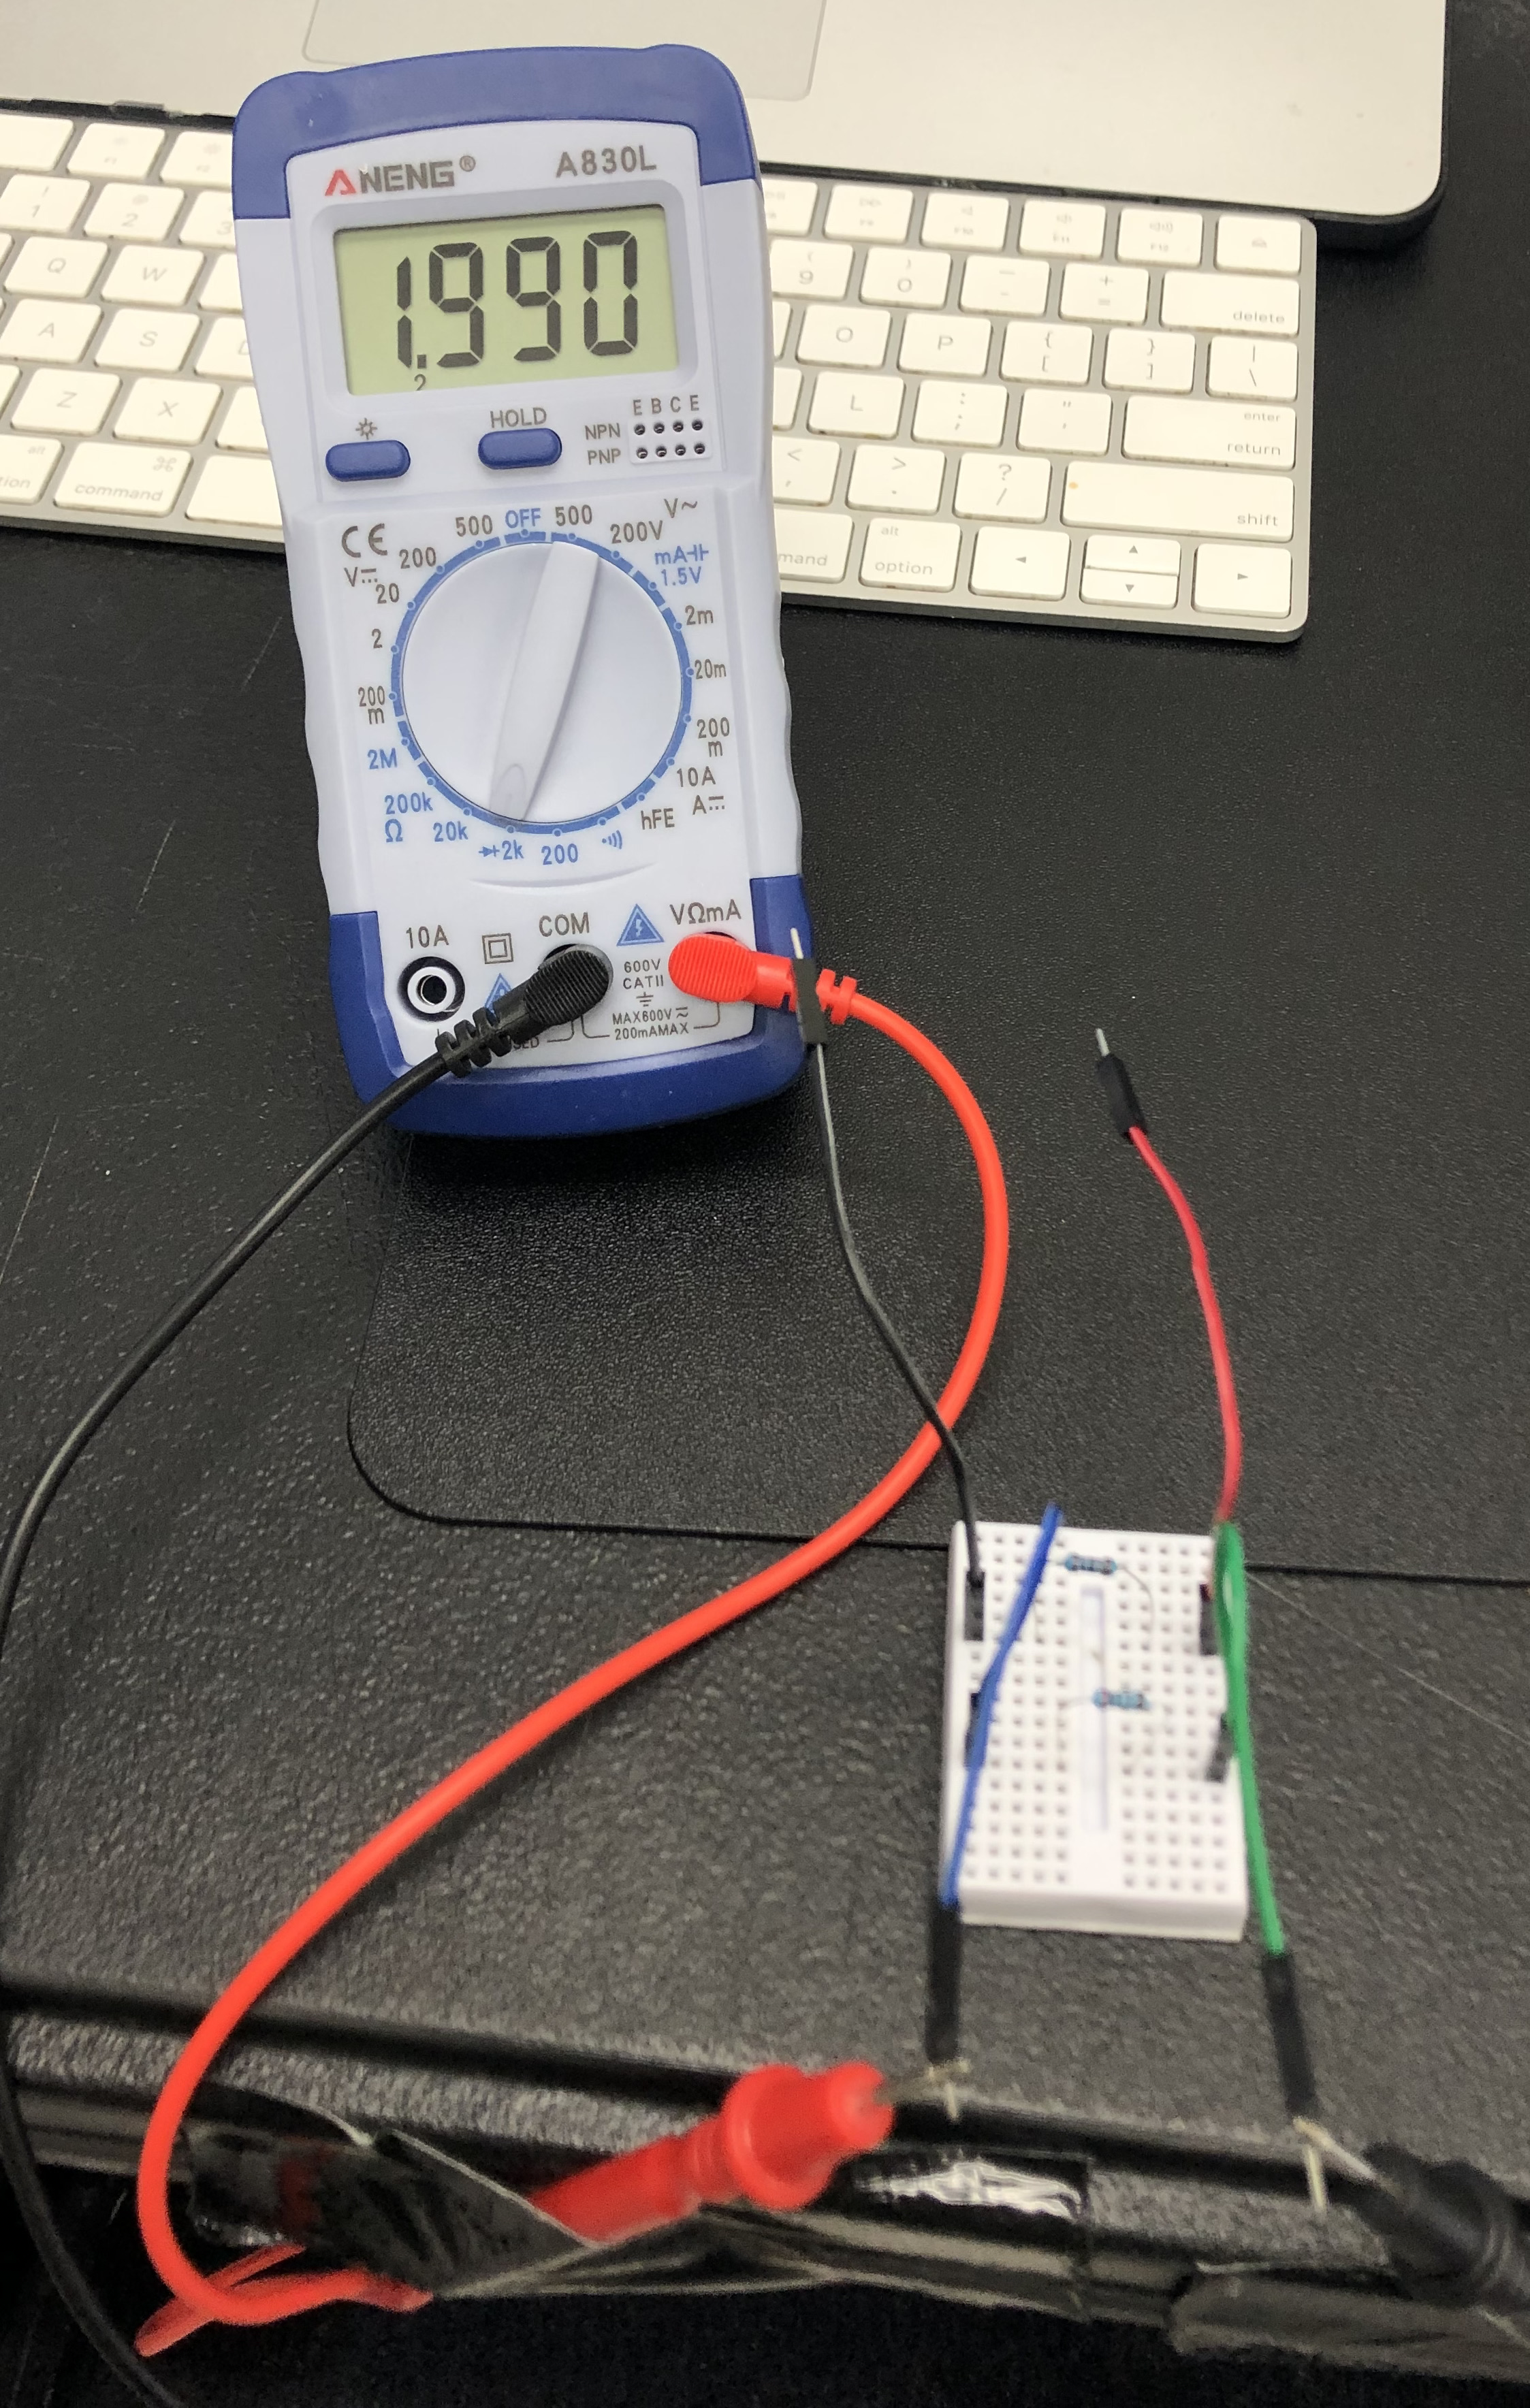
\includegraphics[scale=0.070,height=4.5cm]{R2.jpeg}
    \subsection*{Graph 1}
    % 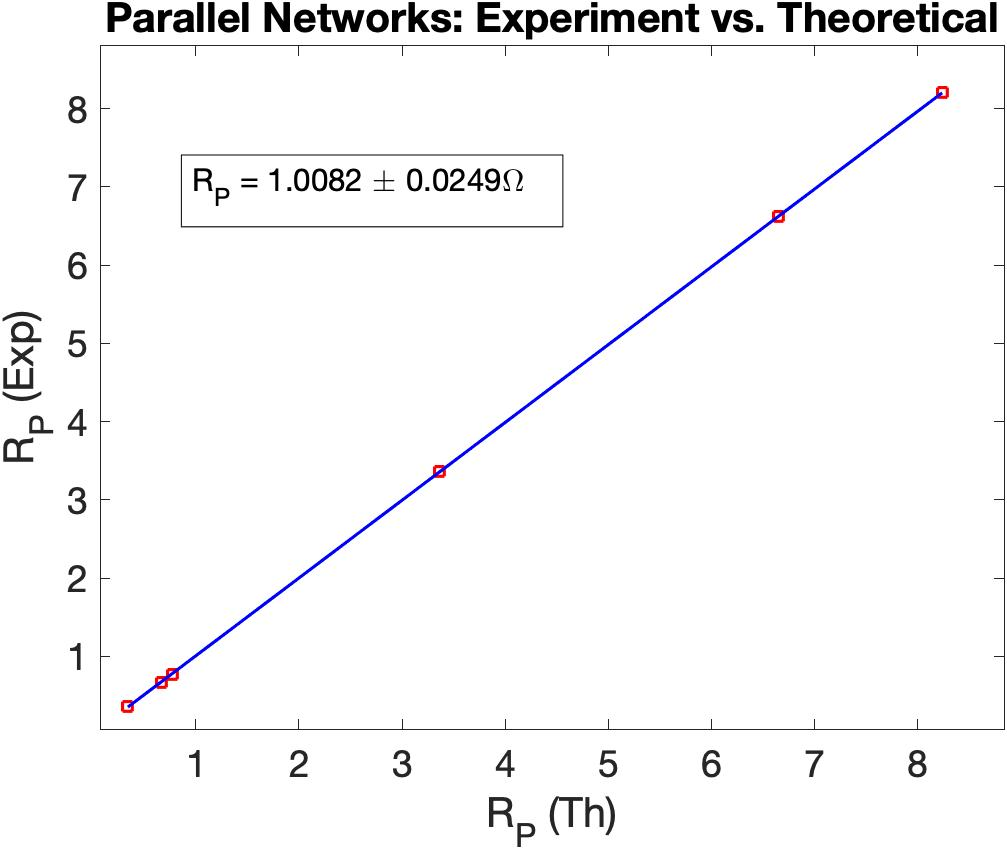
\includegraphics[scale=0.18]{parallel.jpeg}
    \subsection*{Discussion 1}
    \begin{enumerate}
      \item What did you expect to see, and did you see it? If not, why not. If so, how well (quantitatively) did it fit your expectation?
      \begin{itemize}
        \item
      \end{itemize}
    \end{enumerate}
  \end{center}
\end{table}
\newpage
\begin{table}[!htp]\centering
  \subsection*{Part 2}
  \begin{tabular}{|c|c|c|c|c|c|c|c|c|c|c|}\hline
  \multicolumn{10}{|c|}{\textbf{Table 2: Parallel Resistors}} \\\hline
  \R{1} & \R{2} & \R{3} & \V{1} & V/DIV for \V{1} &  \I{1} = \I{23} & \V{123} & \V{23} & \R{23,expt} & \R{23,theory} \\\hline
  1k & 2k & 0 & 0 & 0 & 0 & 0 & 0 & 0 & 0\\\hline
  1k & 100 & 0 & 0 & 0 & 0 & 0 & 0 & 0 & 0\\\hline
  1k & 4.7k & 0 & 0 & 0 & 0 & 0 & 0 & 0 & 0\\\hline
  1k & 10k & 0 & 0 & 0 & 0 & 0 & 0 & 0 & 0\\\hline
  1k & 100k & 0 & 0 & 0 & 0 & 0 & 0 & 0 & 0\\\hline
  \end{tabular}
  \begin{center}
    \subsection*{Picture 2: }
    % 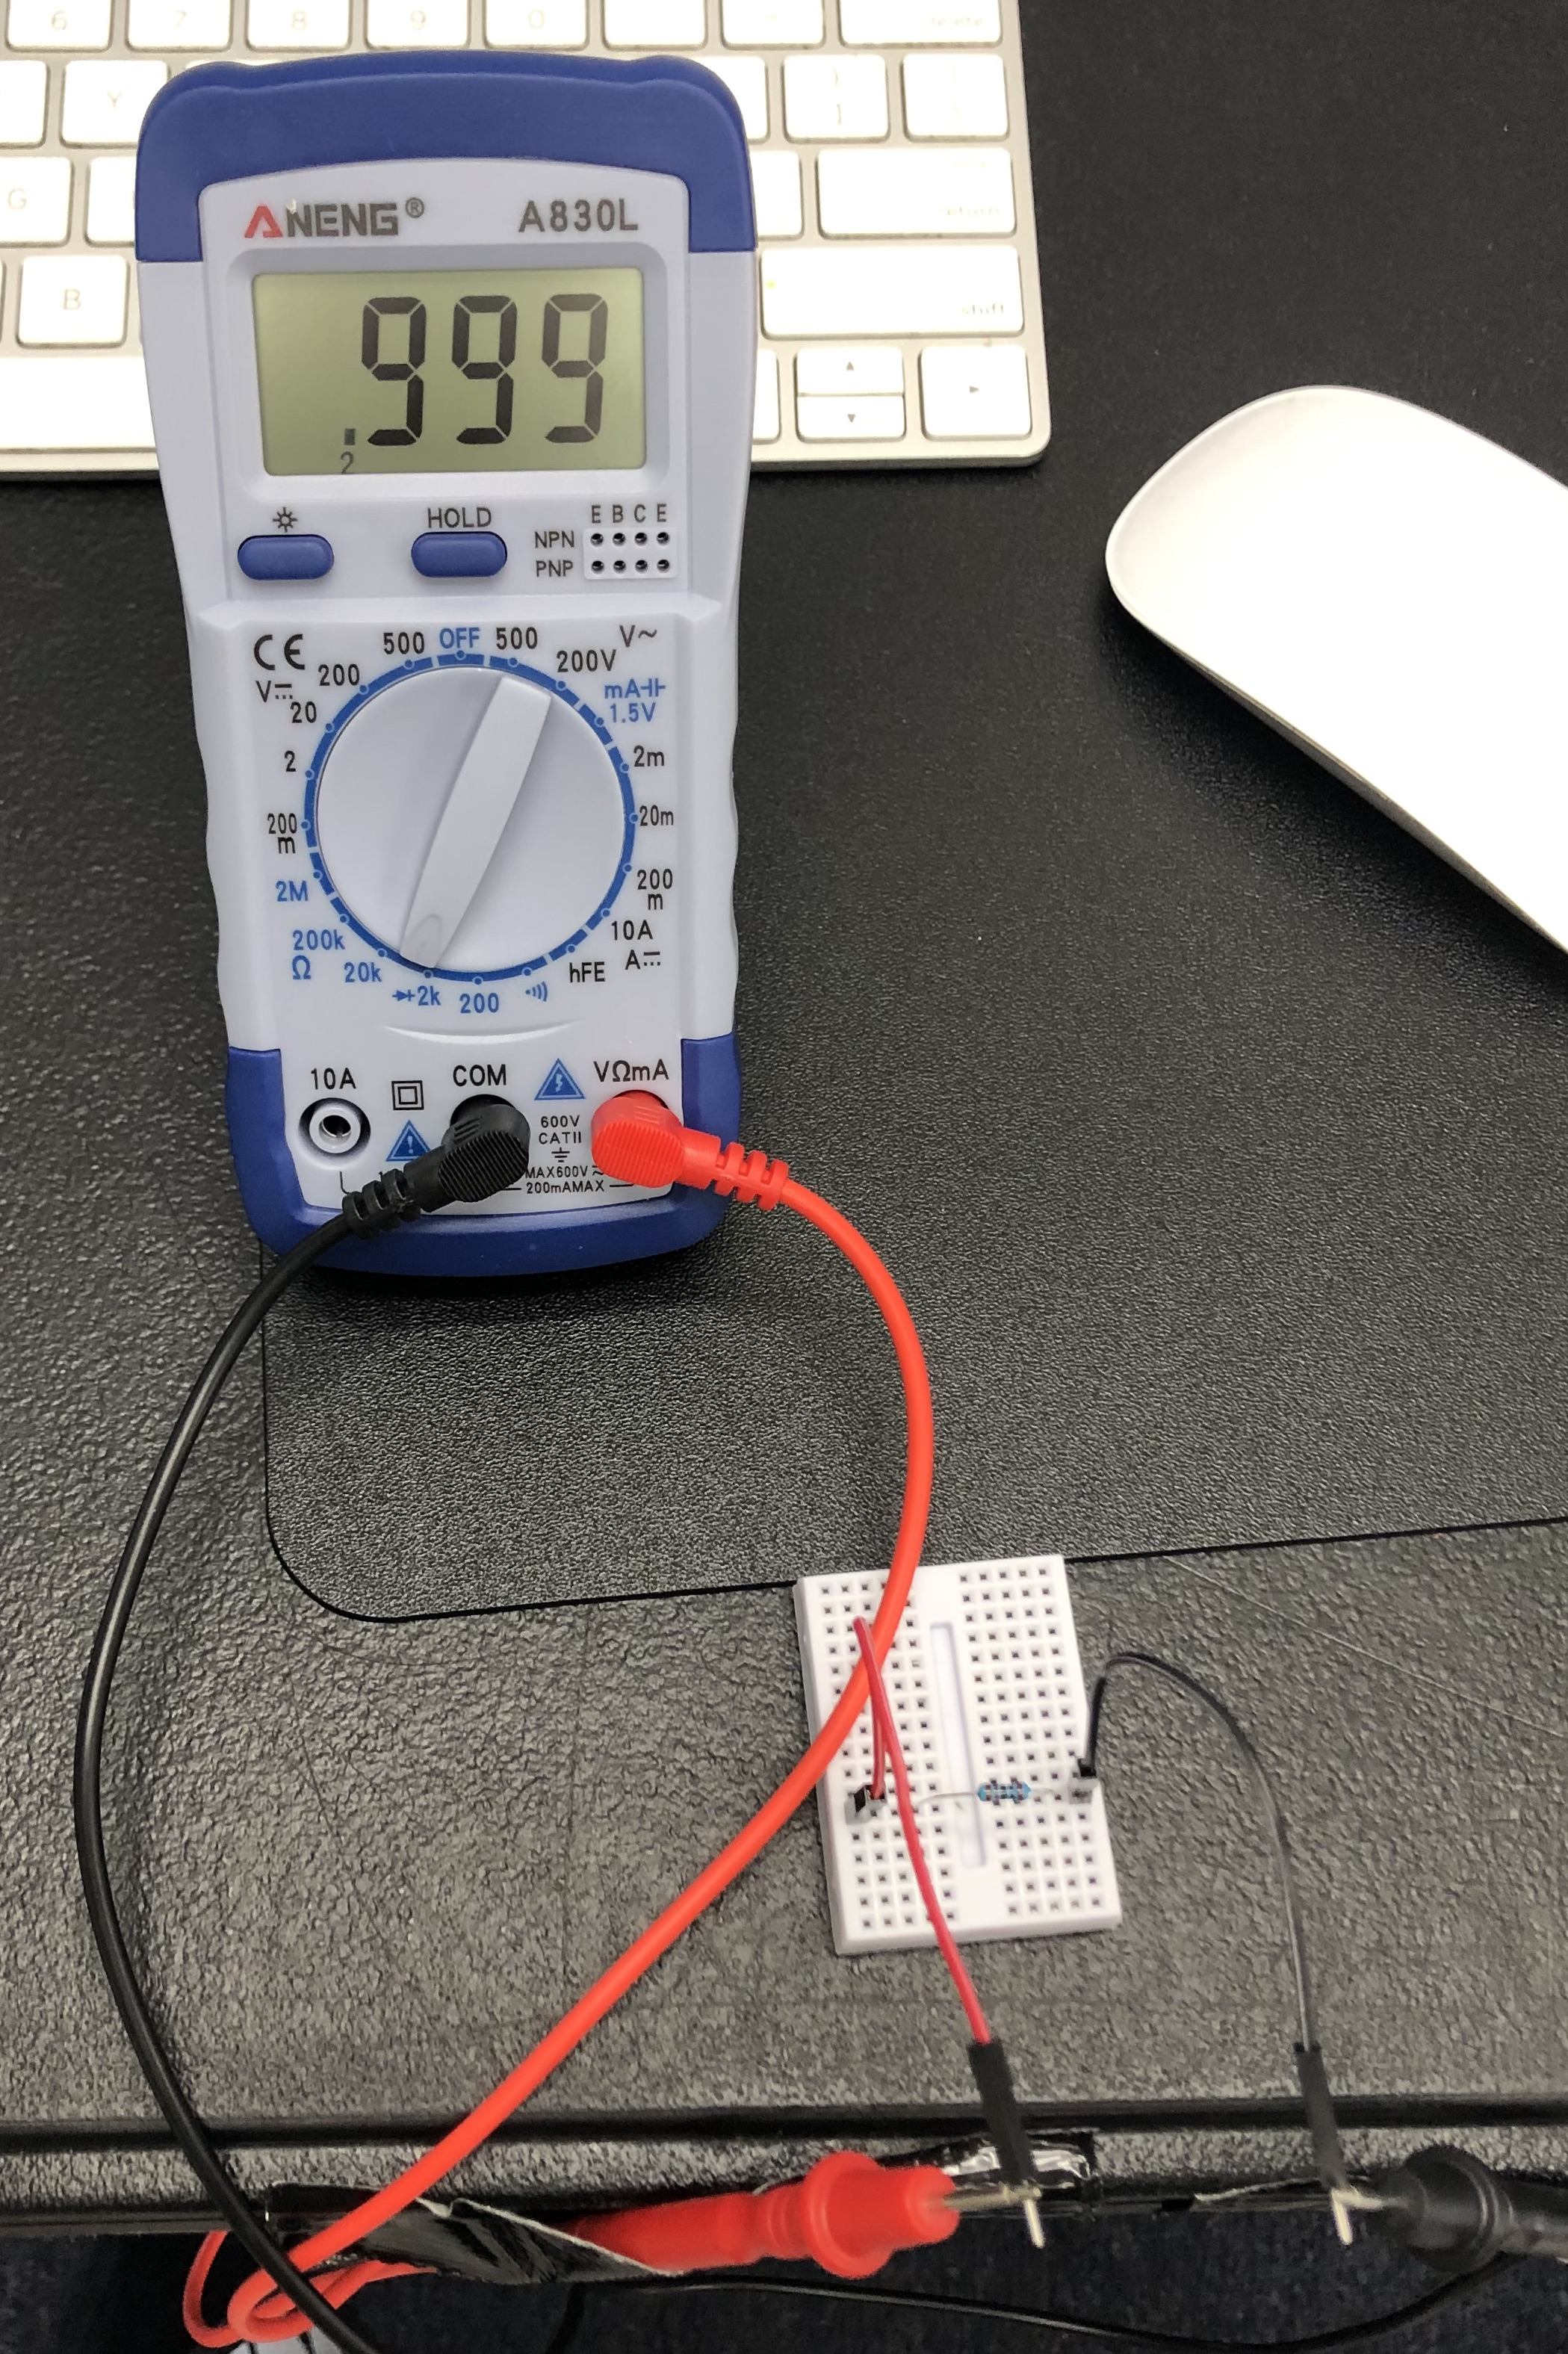
\includegraphics[scale=0.079,height=4.5cm]{R1.jpeg}
    % 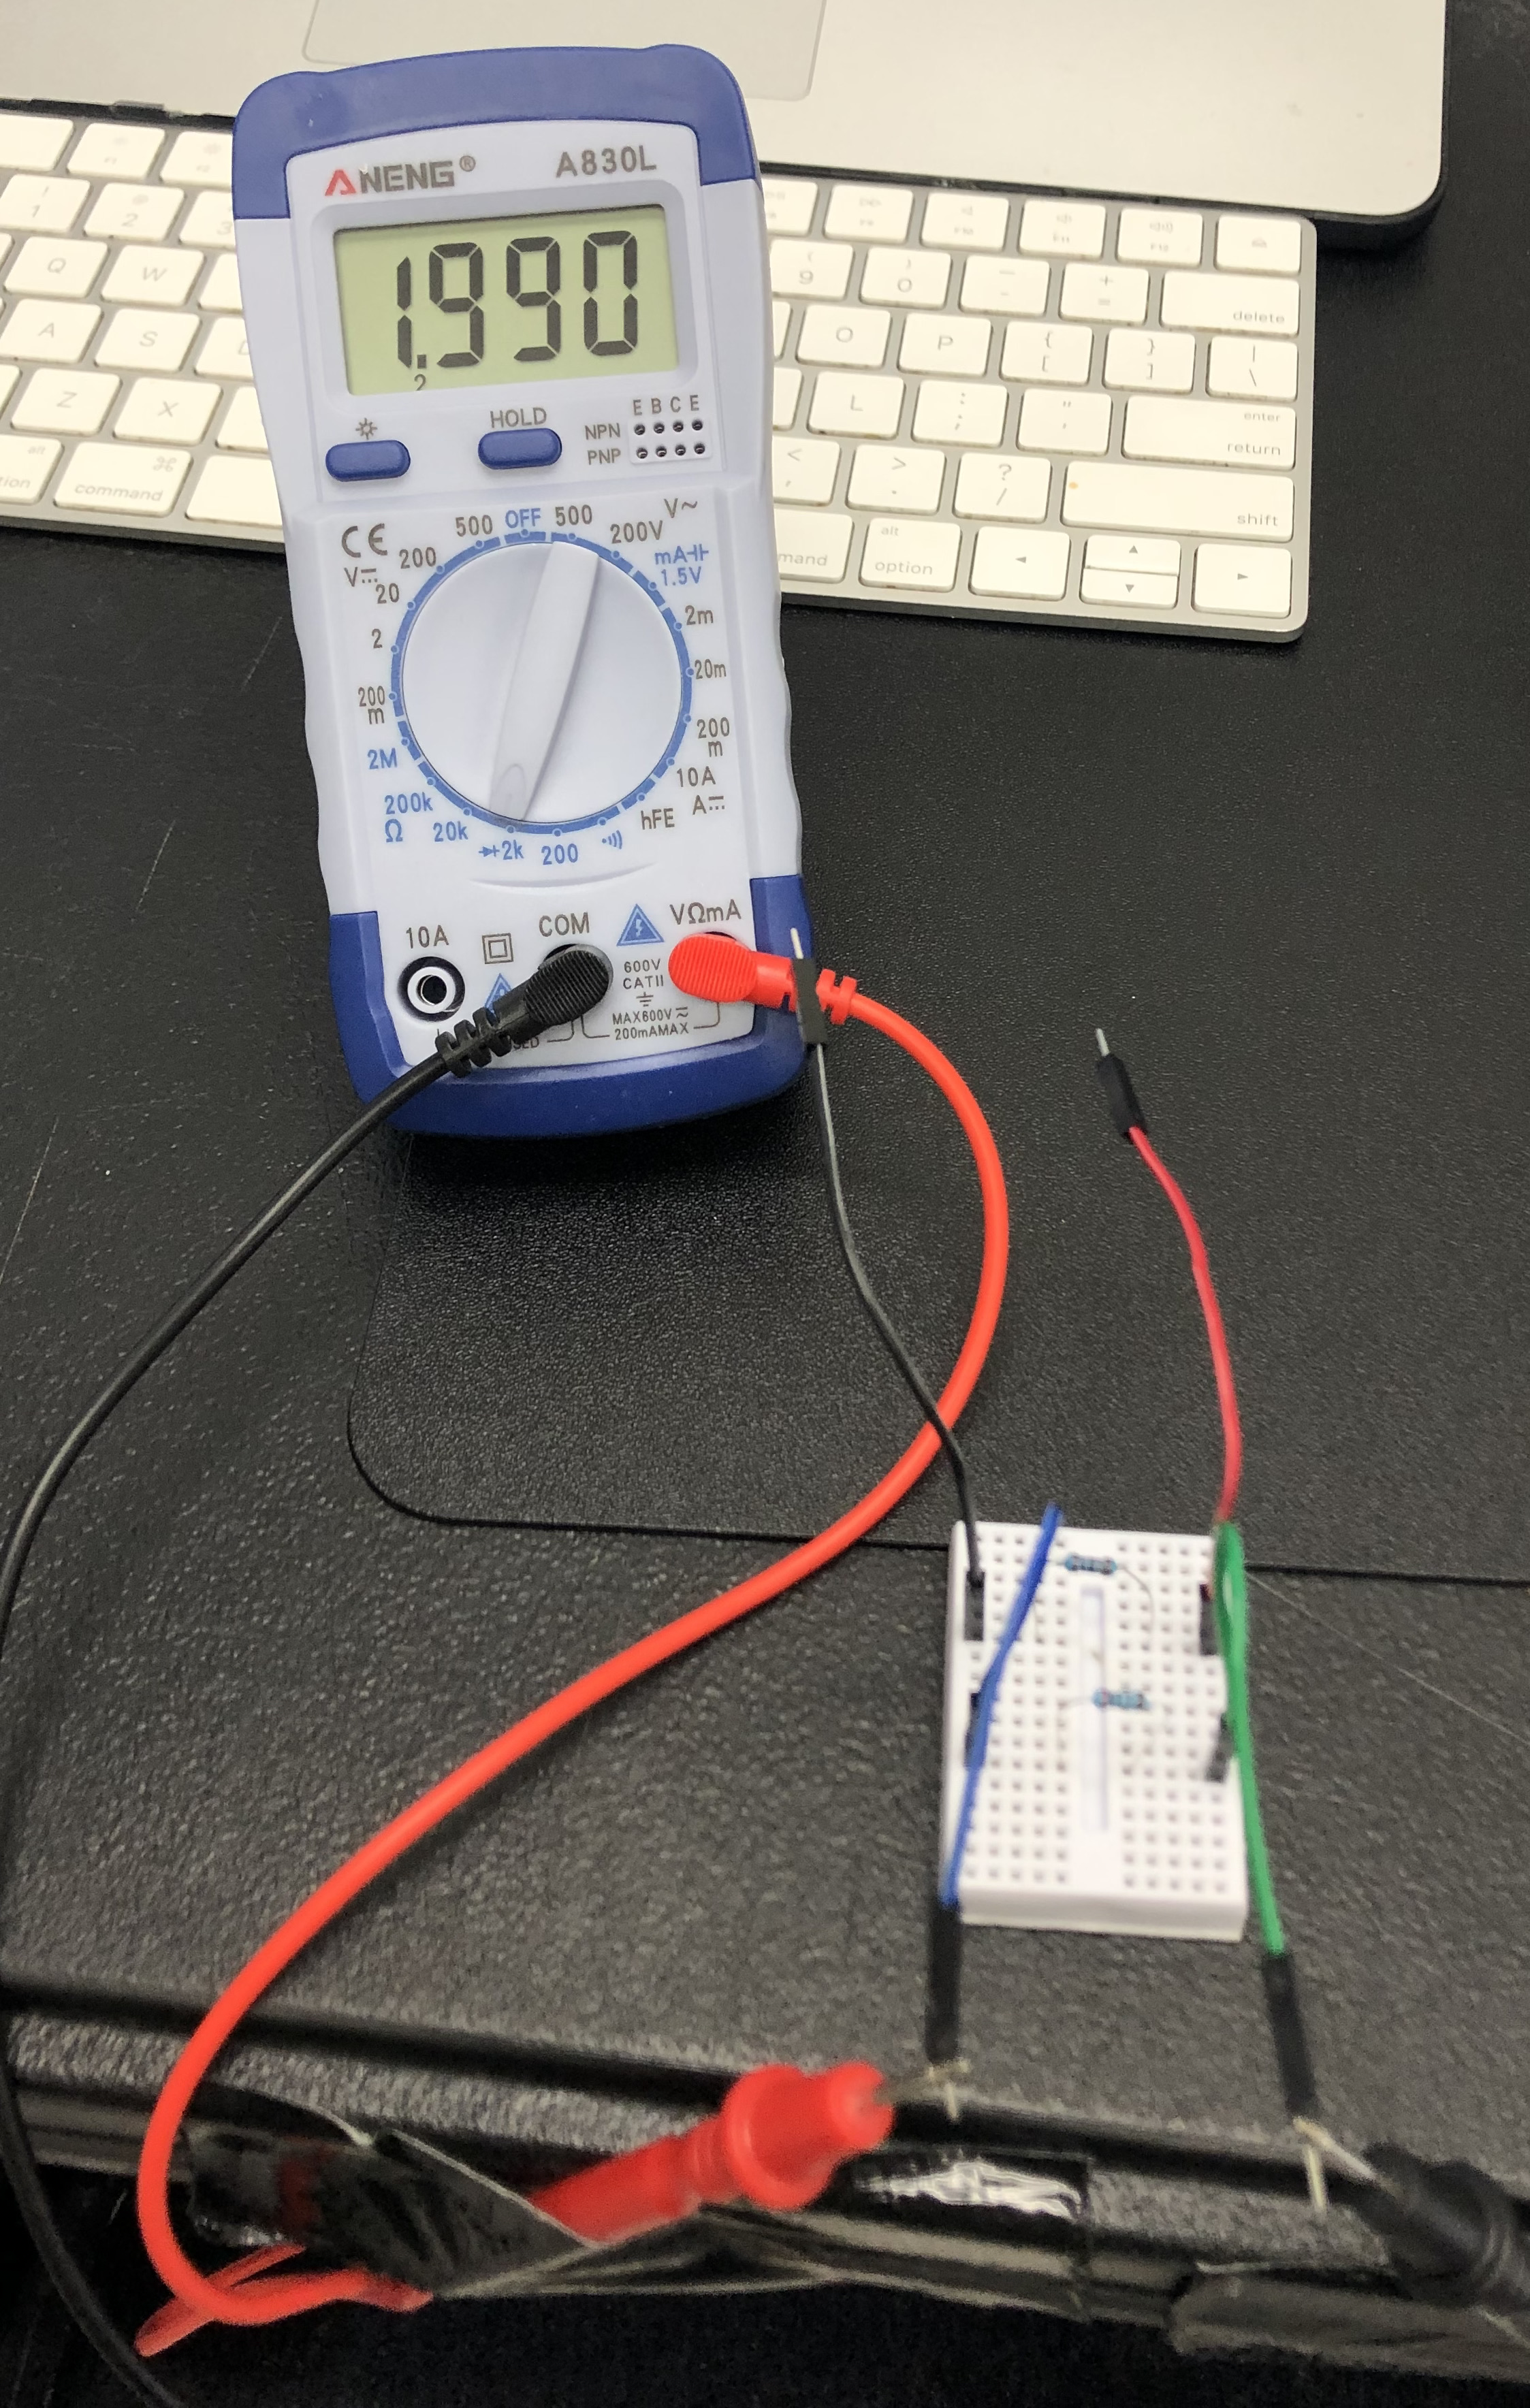
\includegraphics[scale=0.070,height=4.5cm]{R2.jpeg}
    \subsection*{Graph 2}
    % 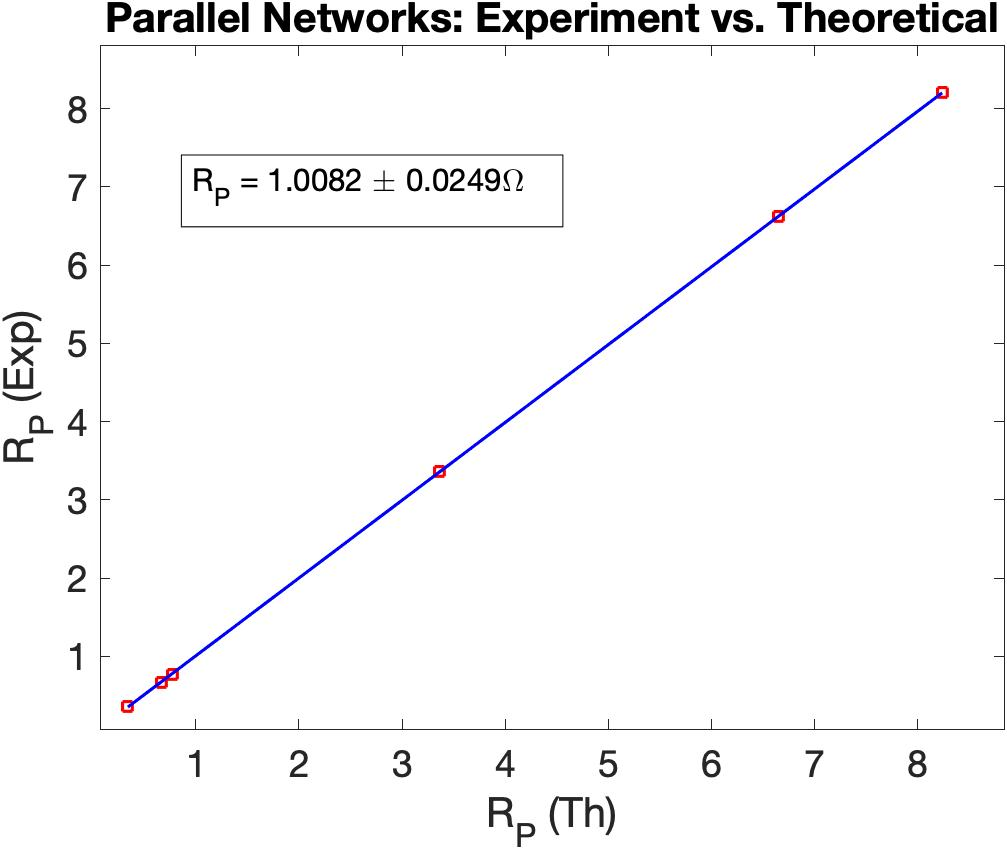
\includegraphics[scale=0.18]{parallel.jpeg}
    \subsection*{Discussion 2}
    \begin{enumerate}
      \item What did you expect to see, and did you see it? If not, why not. If so, how well (quantitatively) did it fit your expectation?
      \begin{itemize}
        \item
      \end{itemize}
    \end{enumerate}
  \end{center}
\end{table}
\end{document}
